\documentclass[11pt, twoside]{article}

\usepackage{fancyhdr} % Required for custom headers
\usepackage{lastpage} % Required to determine the last page for the footer
\usepackage{extramarks} % Required for headers and footers
\usepackage[usenames,dvipsnames]{color} % Required for custom colors
\usepackage{graphicx} % Required to insert images
\usepackage{listings} % Required for insertion of code
\usepackage{courier} % Required for the courier font
\usepackage{url}
\usepackage{mathptmx} % Times New Roman

%----------------------------------------------------------------------------------------
% Change section style
%----------------------------------------------------------------------------------------
\usepackage{lipsum, graphicx, tabularx}
\usepackage[svgnames]{xcolor}
\usepackage[explicit]{titlesec}
\titleformat{\section}[block]
    {\bfseries\Huge\sffamily}
    {\rlap{\hspace*{\dimexpr\linewidth-5 \marginparsep}%
    \begin{tabular}{@{}>{\color{gray!90}}c@{}}\scalebox{4}{\thesection}\\[-1.3ex]%
    \rule{10pt}{10pt}\hspace{10pt}\rule{10pt}{10pt}\hspace{10pt}\rule{10pt}{10pt}\end{tabular}}}
    {0pt}
    {\color{gray!75}\begin{tabularx}{\dimexpr\linewidth+4\marginparsep}%
    {@{}>{\raggedright\arraybackslash}X>{\raggedleft\arraybackslash}r@{}}
       & \rule{0pt}{3ex}\\[0ex] #1
    \end{tabularx}}
    [\vspace{1ex}\titlerule\vspace{16pt}]

\titlespacing{\chapter}{0pt}{-5ex}{10ex}


%----------------------------------------------------------------------------------------
%	SPANISH LANGUAGE
%----------------------------------------------------------------------------------------
\usepackage{lmodern}
\usepackage[T1]{fontenc}
\usepackage[spanish,activeacute]{babel}
\usepackage[utf8]{inputenc} % Para poder incluir tildes y ñ automáticamente

%----------------------------------------------------------------------------------------
%	TODOs AND NOTES
%----------------------------------------------------------------------------------------

\usepackage{xargs}                      % Use more than one optional parameter in a new commands
\usepackage[colorinlistoftodos,prependcaption,textsize=tiny]{todonotes}
\newcommandx{\unsure}[2][1=]{\todo[linecolor=red,backgroundcolor=red!25,bordercolor=red,#1]{#2}}
\newcommandx{\change}[2][1=]{\todo[linecolor=blue,backgroundcolor=blue!25,bordercolor=blue,#1]{#2}}
\newcommandx{\info}[2][1=]{\todo[linecolor=OliveGreen,backgroundcolor=OliveGreen!25,bordercolor=OliveGreen,#1]{#2}}
\newcommandx{\improvement}[2][1=]{\todo[linecolor=Plum,backgroundcolor=Plum!25,bordercolor=Plum,#1]{#2}}
\newcommandx{\thiswillnotshow}[2][1=]{\todo[disable,#1]{#2}}

%----------------------------------------------------------------------------------------
%	MARGIN, HEADER AND FOOTER
%----------------------------------------------------------------------------------------
% Margins
\usepackage{lipsum}

\topmargin=-0.45in
\evensidemargin=0in
\oddsidemargin=0in
\textwidth=6.5in
\textheight=9.0in
\headsep=0.25in

\linespread{1.1} % Line spacing

% Set up the header and footer
\fancypagestyle{insection}{
\fancyhf{}
\fancyfoot[C]{[ \textbf{\thepage}   ]}
\renewcommand{\headrulewidth}{0pt}
\renewcommand{\footrulewidth}{1pt}
}

% First section page
\fancypagestyle{notsection}{

\fancyhead[LE,RO]{\textbf{\leftmark}}
\fancyhead[LO,RE]{[ \textbf{\thepage}   ]}
\fancyfoot[CE,LE,RE,CO,LO,RO]{}
\renewcommand{\headrulewidth}{1pt}
\renewcommand{\footrulewidth}{0pt}
}

\setlength\parindent{0pt} % Removes all indentation from paragraphs


%----------------------------------------------------------------------------------------
%	INFO BOXES
%----------------------------------------------------------------------------------------
\usepackage[tikz]{bclogo}
\usepackage[framemethod=tikz]{mdframed}
\usepackage[many]{tcolorbox}

\definecolor{bgblue}{RGB}{245,243,253}
\definecolor{ttblue}{RGB}{91,194,224}


\newtcolorbox{normalbox}[1][]{
  breakable,
  title=#1,
  colback=white,
  colbacktitle=white,
  coltitle=black,
  fonttitle=\center\bfseries,
  bottomrule=0pt,
  toprule=0pt,
  leftrule=3pt,
  rightrule=3pt,
  titlerule=0pt,
  arc=0pt,
  outer arc=0pt,
  colframe=black,
}

\newtcolorbox{greenbox}[1][]{
  breakable,
  freelance,
  title=#1,
  colback=green!10,
  colbacktitle=green!10,
  coltitle=black,
  fonttitle=\center\bfseries,
  bottomrule=0pt,
  boxrule=0pt,
  colframe=white,
  overlay unbroken and first={
  \draw[green!75!black,line width=3pt]
    ([xshift=5pt]frame.north west) -- 
    (frame.north west) -- 
    (frame.south west);
  \draw[green!75!black,line width=3pt]
    ([xshift=-5pt]frame.north east) -- 
    (frame.north east) -- 
    (frame.south east);
  },
  overlay unbroken app={
  \draw[green!75!black,line width=3pt,line cap=rect]
    (frame.south west) -- 
    ([xshift=5pt]frame.south west);
  \draw[green!75!black,line width=3pt,line cap=rect]
    (frame.south east) -- 
    ([xshift=-5pt]frame.south east);
  },
  overlay middle and last={
  \draw[green!75!black,line width=3pt]
    (frame.north west) -- 
    (frame.south west);
  \draw[green!75!black,line width=3pt]
    (frame.north east) -- 
    (frame.south east);
  },
  overlay last app={
  \draw[red!75!black,line width=3pt,line cap=rect]
    (frame.south west) --
    ([xshift=5pt]frame.south west);
  \draw[red!75!black,line width=3pt,line cap=rect]
    (frame.south east) --
    ([xshift=-5pt]frame.south east);
  },
}


%----------------------------------------------------------------------------------------
%	CODE INCLUSION CONFIGURATION
%----------------------------------------------------------------------------------------
\definecolor{gray97}{gray}{.97}
\definecolor{gray75}{gray}{.75}
\definecolor{gray45}{gray}{.45}
\definecolor{comments}{RGB}{0,100,0}

\lstset{ frame=Ltb,
     framerule=0pt,
     aboveskip=0.5cm,
     framextopmargin=3pt,
     framexbottommargin=3pt,
     framexleftmargin=0.4cm,
     framesep=0pt,
     rulesep=.4pt,
     backgroundcolor=\color{gray97},
     %
     stringstyle=\ttfamily\color{comments},
     showstringspaces = false,
     basicstyle=\footnotesize\ttfamily,
     commentstyle=\itshape\color{gray45},
	 keywordstyle=\bfseries\color{blue},
     %
     numbers=left,
     numbersep=15pt,
     numberstyle=\tiny,
     numberfirstline = false,
     breaklines=true,
   }
   
\lstdefinestyle{ConfigFiles}{% define own style
  language={[LaTeX]TeX},
  basicstyle=\small\ttfamily,
  linewidth=0.9\linewidth,
  breaklines=true,
  keywordstyle=\color{blue}\bfseries,
  identifierstyle=\color{orange},
  commentstyle=\color{cyan},
  backgroundcolor=\color{OliveGreen},
  tabsize=2,
  morekeywords = {parameter},
}

\lstdefinestyle{consola}
   {basicstyle=\scriptsize\bf\ttfamily,
    backgroundcolor=\color{gray75},
   }
 
\lstdefinestyle{C}
   {language=C,
   }


\begin{document}
\begin{titlepage}
\begin{center}
\vspace*{-1in}
\begin{figure}[htb]
\begin{center}

\includegraphics[width=5cm]{./images/uclm_logo.eps} 
\hspace*{1.5in}

\includegraphics[width=5cm]{./images/esi_logo.eps}
\end{center}
\end{figure}
\end{center}
\begin{center}
UCLM - Escuela Superior de Informática - Ciudad Real\\
\vspace*{0.6in}
\vspace*{0.2in}
\begin{Large}
\textbf{Curso de Experto en Desarrollo de Videojuegos} \\
\textbf{\textit{Primera Entrega}} \\
\end{Large}
\vspace*{0.3in}
\vspace*{0.3in}
\rule{80mm}{0.1mm}\\
\vspace*{0.1in}
\begin{large}
Hecho por: \\
Javier Córdoba Romero \\
Juan José Corroto Martín \\
Iván García Herrera \\
\vspace*{0.3in}
Fecha: Junio de 2018.\\
\end{large}
\end{center}

\end{titlepage}
\tableofcontents
% cuerpo del documento
\newpage

\pagestyle{insection}
\section{Título}
\markboth{Título}{}

\textbf{Alliance}.

\pagestyle{insection}
\section{Autores}
\markboth{Autores}{}
Javier Córdoba Romero. \\
Juan José Corroto Martín. \\
Iván García Herrera.

\pagestyle{insection}
\section{Descripción breve}
\markboth{Descripción breve}{}

Juego de acción en tercera persona dividido en 2 niveles. El juego consistirá en avanzar en la trama de la historia, estando cada punto importante encerrado detrás de una pelea contra un boss. Algunas puertas tendrán que ser \textit{``hackeadas''} para poder avanzar, siendo este \textit{hackeo} la resolución de un minijuego de tipo puzzle. En el primer nivel, cada punto importante de la historia aumentará el tamaño de nuestro grupo, siendo cada integrante un NPC. El juego dará la opción de elegir a uno de los dos personajes iniciales, cada uno con un tipo distinto de combate. Cada personaje tendrá 2 tipos distintos de ataque, siendo posible hacer combos entre cada uno de ellos. Además tendrá la opción de jugar en modo cooperativo local, controlando el otro personaje el segundo jugador.

\pagestyle{insection}
\section{Lista de descriptores}
\markboth{Lista de descriptores}{}
\begin{itemize}
\item Acción.
\item Tercera Persona.
\item Peleas con bosses.
\item Cooperativo.
\item Minijuego.
\item Historia lineal.
\end{itemize}

\pagestyle{insection}
\section{Requisitos específicos que ha de \\ cumplir el desarrollo}
\markboth{Requisitos específicos que ha de cumplir el desarrollo}{}

\subsection{Requisitos Funcionales}


\subsection{Requisitos No Funcionales}

\pagestyle{insection}
\section{Dinámica del juego}
\markboth{Título}{}


\subsection{Argumento}
Eres \textit{Alyssa Theras} parte de la poca resistencia que queda en el planeta Tierra. Habéis sido invadidos por una raza extraterrestre que quiere esclavizaros. Tu misón será encontrar a otros miembros de la resistencia y unir fuerzas con ellos para liberar a la Tierra del invasor enemigo. 

\subsection{Jugadores}
Se trata de un juego de un solo jugador con posibilidad de campaña cooperativa de dos jugadores en forma remota. El jugador principal podrá elegir si quiere jugar con \textit{Alyssa} o con \textit{Morten}. Si un segundo jugador se une a la partida, controlará al otro personaje.

\pagestyle{insection}
\subsection{Personajes}
\markboth{Personajes}{}

\subsubsection{\textit{Alyssa Theras}}
\begin{itemize}
\item \textbf{Historia pasada:} \textit{Alyssa} es una soldado superviviente en la primera guerra interplanetaria. Vio morir a todos sus compañeros y por eso odia la violencia, pero a la vez se siente obligada por ser una de las únicas personas que no están esclavizadas. 
\item \textbf{Objetivos:} conseguir la paz mediante la liberación de los esclavos y eliminación de los enemigos invasores.
\item \textbf{Armas:} Su arma principal será una maza, aunque también es diestra con las armas a distancia. 
\end{itemize}

\begin{center}
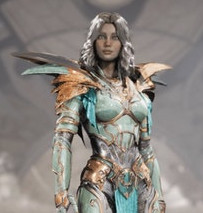
\includegraphics[width=5cm]{./images/alyssa.jpg}
\end{center}

\subsubsection{\textit{Morten Vengeance}}
\begin{itemize}
\item \textbf{Historia pasada:} \textit{Morten} fue un compañero de \textit{Alyssa} en la guerra interplanetaria y también vio morir a todos sus compañeros. Sin embargo está enfadado con el mundo y quiere que sus enemigos paguen por lo que han hecho. 
\item \textbf{Objetivos:} ayudar a \textit{Alyssa} a eliminar a sus enemigos sin piedad. 
\item \textbf{Armas:} Sus armas principales son dos pistolas aunque también se maneja con artillería pesada. 
\end{itemize}

\begin{center}
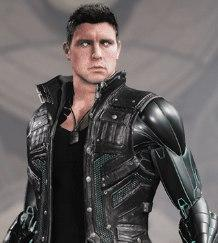
\includegraphics[width=4cm]{./images/morten.jpg}
\end{center}

\subsubsection{\textit{Serj Mao}}
\begin{itemize}
\item \textbf{Historia pasada:} \textit{Serj} fue un general del bando contrario a \textit{Alyssa} en la guerra interplanetaria. Ahora es solo un esclavo a las órdenes de la raza alienígena.
\item \textbf{Objetivos:} cuando conoce a \textit{Alyssa} le cuenta su plan y se decide a ayudarla. 
\item \textbf{Armas:} Su arma principal es una lanza \textit{Guan dao}.
\end{itemize}

\pagestyle{notsection}

\begin{center}
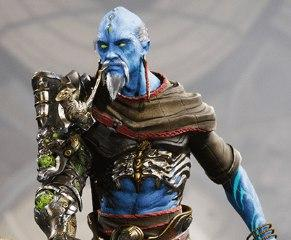
\includegraphics[width=5cm]{./images/serj.jpg}
\end{center}

\subsubsection{\textit{Spectre}}
\begin{itemize}
\item \textbf{Historia pasada:} \textit{Spectre} es una experta \textit{hacker} que trabajaba de administradora de sistemas. Como esclava está muy en alta estima por sus captores gracias a sus conocimientos técnicos y vive bien. 
\item \textbf{Objetivos:} \textit{hackear} el servidor que debilitará a los enemigos.
\item \textbf{Armas:} Su arma principal es \textit{hackear} a los enemigos a distancia, aunque luchará con los puños si es necesario.
\end{itemize}

\begin{center}
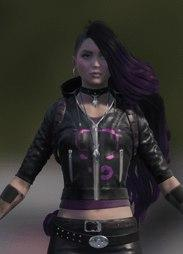
\includegraphics[width=4cm]{./images/spectre.jpg}
\end{center}

\subsubsection{\textit{Henkka}}
\begin{itemize}
\item \textbf{Historia pasada:} \textit{Henkka} es el jefe de los esclavos de la primera zona.
\item \textbf{Objetivos:} eliminar a los revelados.
\item \textbf{Armas:} usa dos armas cuerpo a cuerpo grandes y sus ataques son lentos y contundentes. 
\end{itemize}

\begin{center}
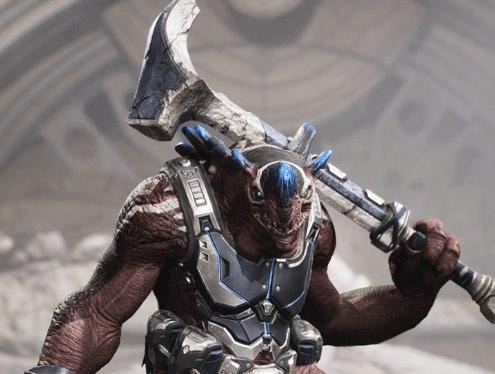
\includegraphics[width=6cm]{./images/henkka.jpg}
\end{center}

\subsubsection{\textit{Euronymous}}
\begin{itemize}
\item \textbf{Historia pasada:} \textit{Euronymous} es el jefe de los esclavos de la segunda zona.
\item \textbf{Objetivos:} eliminar a los revelados.
\item \textbf{Armas:} su arma principal es una espada. Se mueve rápido y puede producir cortes a distancia. 
\end{itemize}

\begin{center}
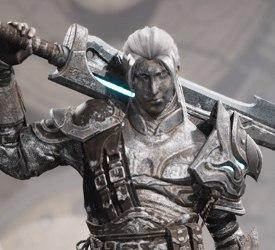
\includegraphics[width=5cm]{./images/euronymous.jpg}
\end{center}

\subsubsection{\textit{Shiva}}
\begin{itemize}
\item \textbf{Historia pasada:} \textit{Shiva} es el jefe de los enemigos alienígenas.
\item \textbf{Objetivos:} defender su nave de los protagonistas para mantener su imperio alienígena.
\item \textbf{Armas:} láser, puños y ataques especiales con los mismos. 
\end{itemize}

\begin{center}
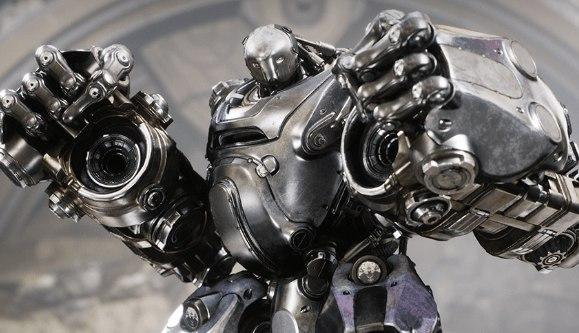
\includegraphics[width=6cm]{./images/shiva.jpg}
\end{center}

\subsubsection{Enemigo guerrero}
\begin{itemize}
\item \textbf{Armas:} principalmente son las hachas.
\item \textbf{Comportamiento:} atacar cuerpo a cuerpo a los protagonistas.
\end{itemize}

\begin{center}
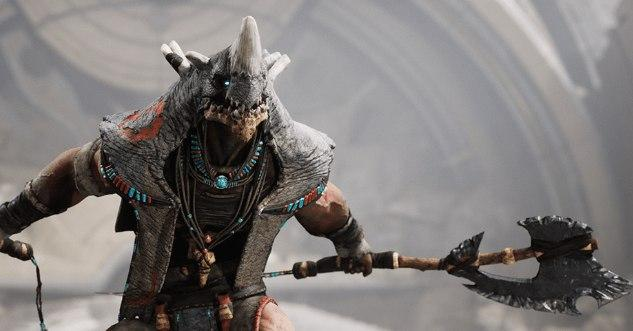
\includegraphics[width=6cm]{./images/guerrero.jpg}
\end{center}

\subsubsection{Enemigo a distancia}
\begin{itemize}
\item \textbf{Armas:} armas de proyectil.
\item \textbf{Comportamiento:} alejarse de los protagonistas y dispararlos.
\end{itemize}

\begin{center}
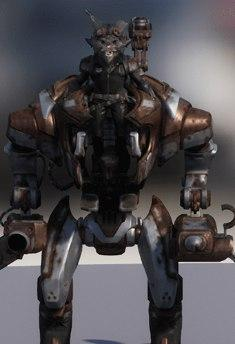
\includegraphics[width=4cm]{./images/distancia.jpg}
\end{center}

\subsubsection{Enemigo tanque}
\begin{itemize}
\item \textbf{Armas:} ataque cuerpo a cuerpo. 
\item \textbf{Comportamiento:} atacar cuerpo a cuerpo con los protagonistas. Puede recibir mucho daño. 
\end{itemize}

\begin{center}
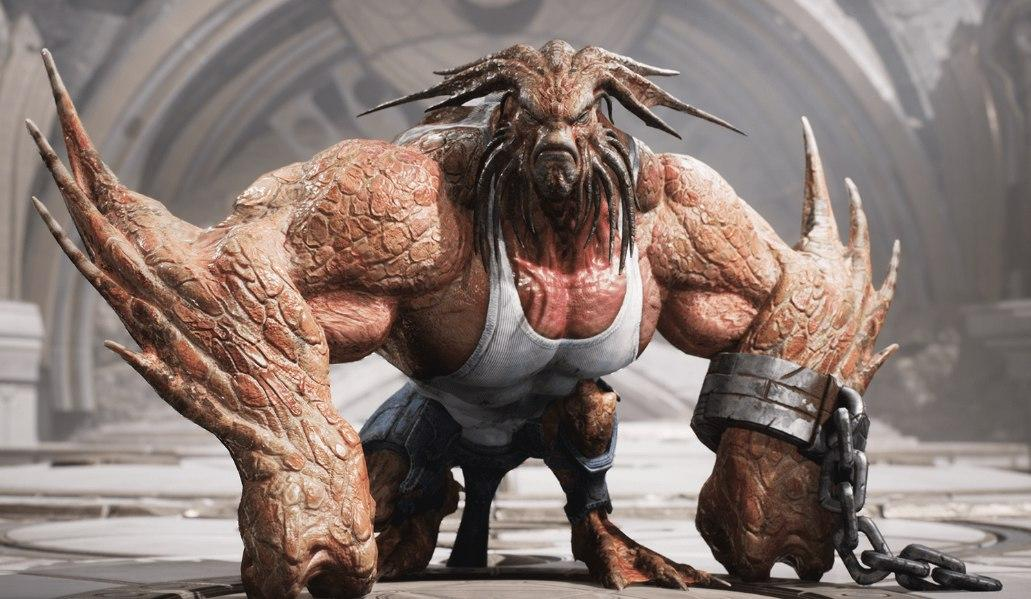
\includegraphics[width=6cm]{./images/tanque.jpg}
\end{center}


\subsection{Historia del mundo}

La trama ocurre en el planeta Tierra, años después de que ocurra una gran guerra contra una raza de otro planeta, la primera guerra interplanetaria. Debido a ella, la población de terrícolas se ha visto disminuida considerablemente y ahora ``conviven'' con su enemigos. Todo esto cambió cuando una raza alienígena llegó a la Tierra junto a su ejército de esclavos para dominarlos. A esta nueva raza no le afectan los ataques terrícolas y nadie sabe el por qué. Por esto, apenas quedan personas y las que quedan son esclavos. 

\subsection{Puntos claves de la historia}

\begin{itemize}
\item El primer punto clave de la historia es la liberación de \textit{Serj}. Antes de aquí te encontrabas sola con \textit{Morten} haciendo guerra de guerrillas para no ser esclavizados. Al liberar a \textit{Serj}, te cuenta que tiene un plan (oye hablar durante su captura de ciertas vulnerabilidades de los enemigos, ya que estos poseen una \texttt{CPU} a modo de cerebro) para deshacerse de los alienígenas. Aceptas y dejas que \textit{Serj} se una a vosotros.
\item Llegados a este punto necesitan a un experto informático que consiga explotar esta vulnerabilidad. Uno de los esclavos liberados cuenta que en ese mismo campamento hay uno, por lo que tu misión es rescatarlo. 
\item Consigues rescatar a tu experta informática (\textit{Spectre}), la cuentas tus pensamientos sobre la vulnerabilidad y ante tu sorpresa, te contesta que es algo que ya sabía pero necesita protección mientras corrompe el código de los enemigos. 
\item Logras infiltrate en la nave enemiga y hay esclavos para detenerte. Mientras te abres paso en la nave, hasta llegar al servidor principal. 
\item En el momento de llegar al servidor princial aparece el jefe final. Luchas con él hasta que \textit{Spectre} consigue hacer al \textit{boss} vulnerable. Vences al jefe final y mientras escapas, los otros enemigos de la misma raza huyen del planeta. 
\end{itemize}


\subsection{Nivel 1.}
La acción tendrá lugar en un bosque. El primer combate contra unos cuantos enemigos servirá como tutorial de mecánicas de combate. Después se avanza hasta un campo de esclavos que van a liberar.Te encuentras con la puerta cerrada donde hay enemigos que tendrás que vencer. Tendrás que encontrar la manera de abrir la puerta (mediante un minijuego, que servirá de tutorial para los distintos minijuegos). Dentro del campamento avanzas y llegas a la plaza de ejecuciones, un área amplia de batalla en la que luchas contra varios enemigos. Hasta que no matas a todos los enemigos, no puedes avanzar. Continúas por una calle hasta que llegas a la entrada de la mina en la cual te encuentras al jefe de los esclavos del campamento, que actúa como primer \textit{boss}. Antes de luchar con él, te envía una oleada de enemigos. Al derrotarlo, habrá una parte de conversación con \textit{Serj} y se continúa el nivel volviendo a la plaza de ejecuciones. A partir de la plaza nos dirigimos al patio de la casa de \textit{Euronymous}, jefe del campamento, que actúa como boss final del nivel. Después, hay un diálogo con \textit{Spectre} donde se forma el plan. 

\subsubsection{Entorno}
Camino dentro de un bosque del que no puedes salir. El campamento estará formado por una parte de bosque y otra de casas de esclavos, de estilo chabola.  La plaza será una zona amplia estilo arena rodeada de casas. La zona del primer \textit{boss} estará en una zona boscosa en la que de lejos verás la entrada de la mina. La zona del boss final estará en otra mini plaza rodeada de casa de esclavos por una parte, una casa más grande por otra parte, rodeada de bosque.

\subsubsection{Enemigos}
Al principio aparecerán sólo guerreros (en el tutorial). En el campamento habrá guerreros y enemigos que atacan a distancia. 

En las calles habrá grupos de enemigos y en la arena y \textit{bosses} vendrán en oleadas.

\subsection{Nivel 2.}

Apareces en una nave espacial, que es la nave de los enemigos alienígenas. Los pasillos son estrechos y hay enemigos patrullando. Entras en un espacio más grande, dónde lucharás con más enemigos y a continuación entrarás a la sala en la que se encuentra el \textit{boss} final. \textit{Spectre} y \textit{Serj} se van de la escena por otro pasillo y los dos protagonistas proceden a luchar contra el \textit{boss}. 

El \textit{boss} es invencible en un principio, y la salud que le quitan los ataques se regenera, por lo que el objetivo es permanecer con vida hasta llegado un cierto punto, en el que \textit{Spectre} avisa que ha logrado \textit{hackear} el sistema de vulnerabilidad. En este punto, el objetivo es eliminar al \textit{boss} final. 

\subsubsection{Entorno}

Pasillos estrechos en el interior de una nave espacial con un estilo futurista. Las habitaciones más grandes son espacios amplios y diáfanos. 

\subsubsection{Enemigos}

Hasta llegar a la zona del \textit{boss} apareceran enemigos de todos los tipos. En los pasillos habrá grupos de enemigos y en el espacio más grande, los enemigos aparecerán en oleadas.

\subsection{Minijuego.}

El juego es el denominado \textbf{``sacar la pieza roja''}. Consiste en mover una serie de bloques sobre una superficie plana para conseguir guiar la pieza principal hacia la salida.


\pagestyle{notsection}

\subsection{Objetivos}

El objetivo del primer nivel se basa en eliminar a los enemigos y conseguir completar tu equipo, para alcanzar con éxito el segundo nivel.

El objetivo del segundo nivel será \textit{hackear} el servidor para hacer que los enemigos alienígenas sean vulnerables al daño humano. 

\subsection{\textit{Gameplay}}

\subsubsection{\textit{Alyssa}}
Puede usar dos armas:
\begin{itemize}
	\item \textbf{Maza:} Tendrá la posibilidad de hacer combos con ataques a corta distancia.
	\item \textbf{Magia:} Podrá lanzar bolas de fuego.
\end{itemize}

\subsubsection{\textit{Morten}}
Puede usar dos armas:
\begin{itemize}
	\item \textbf{Pistolas:} Disparan hacia un enemigo.
	\item \textbf{Granadas:} Proyectil lanzado hacia una localización. Hace daño por explosión. 
\end{itemize}

\newpage
\pagestyle{insection}
\section{Recursos Artístcos}
\markboth{Recursos Artísticos}{}

\subsection{\textit{Assets}}
Todos los assets para personajes y decorado de los mapas han sido sacados principalmente de la tienda del MarketPlace de Epic Games.

\subsection{Bocetos de niveles}
\subsubsection{Nivel1}
\includegraphics[width=16cm]{./images/mapa1.png}

\subsubsection{Nivel2}
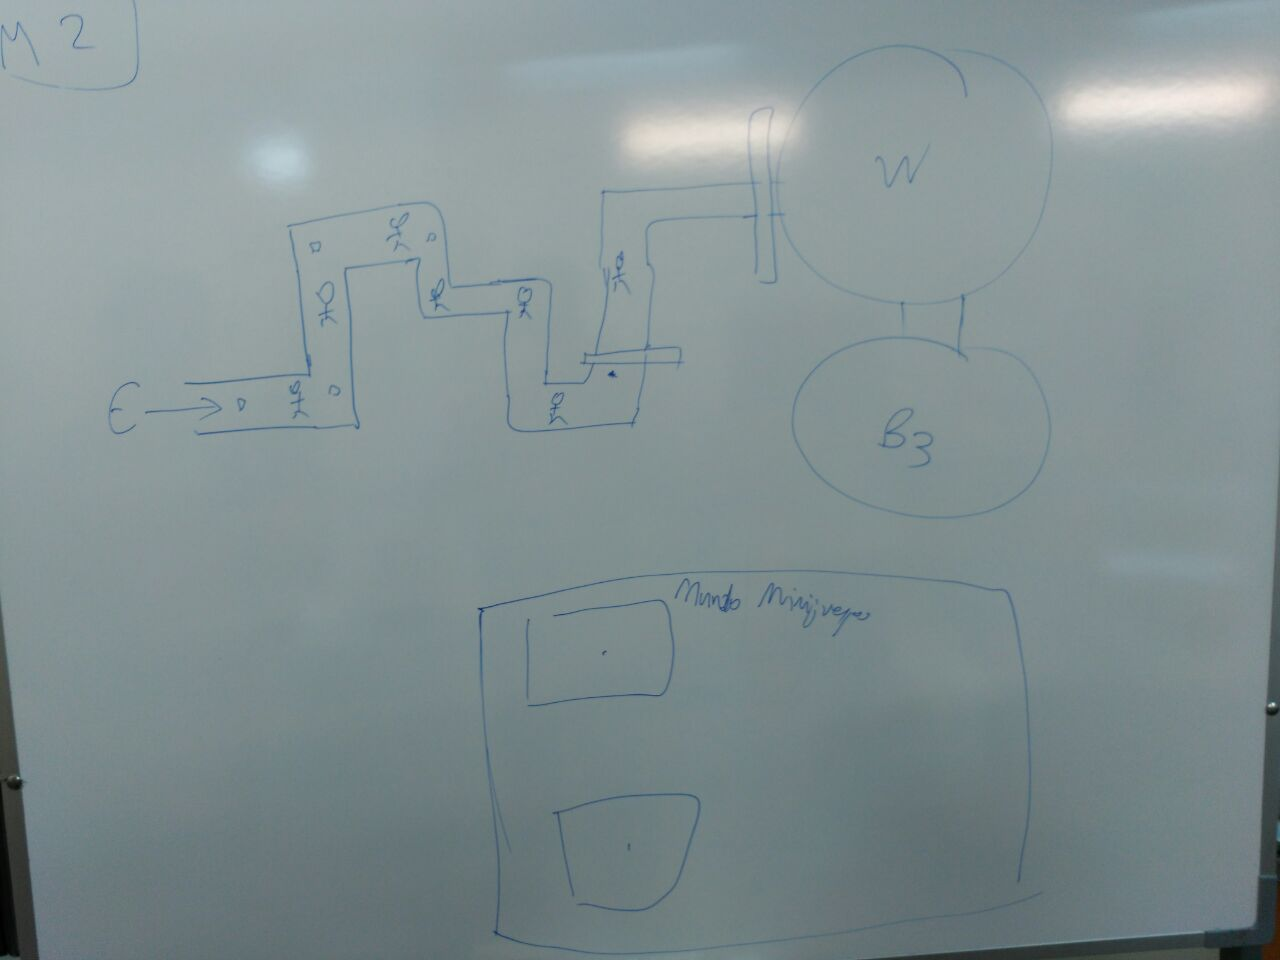
\includegraphics[width=16cm]{./images/Level2.jpg}

\subsection{Bocetos de pantallas}
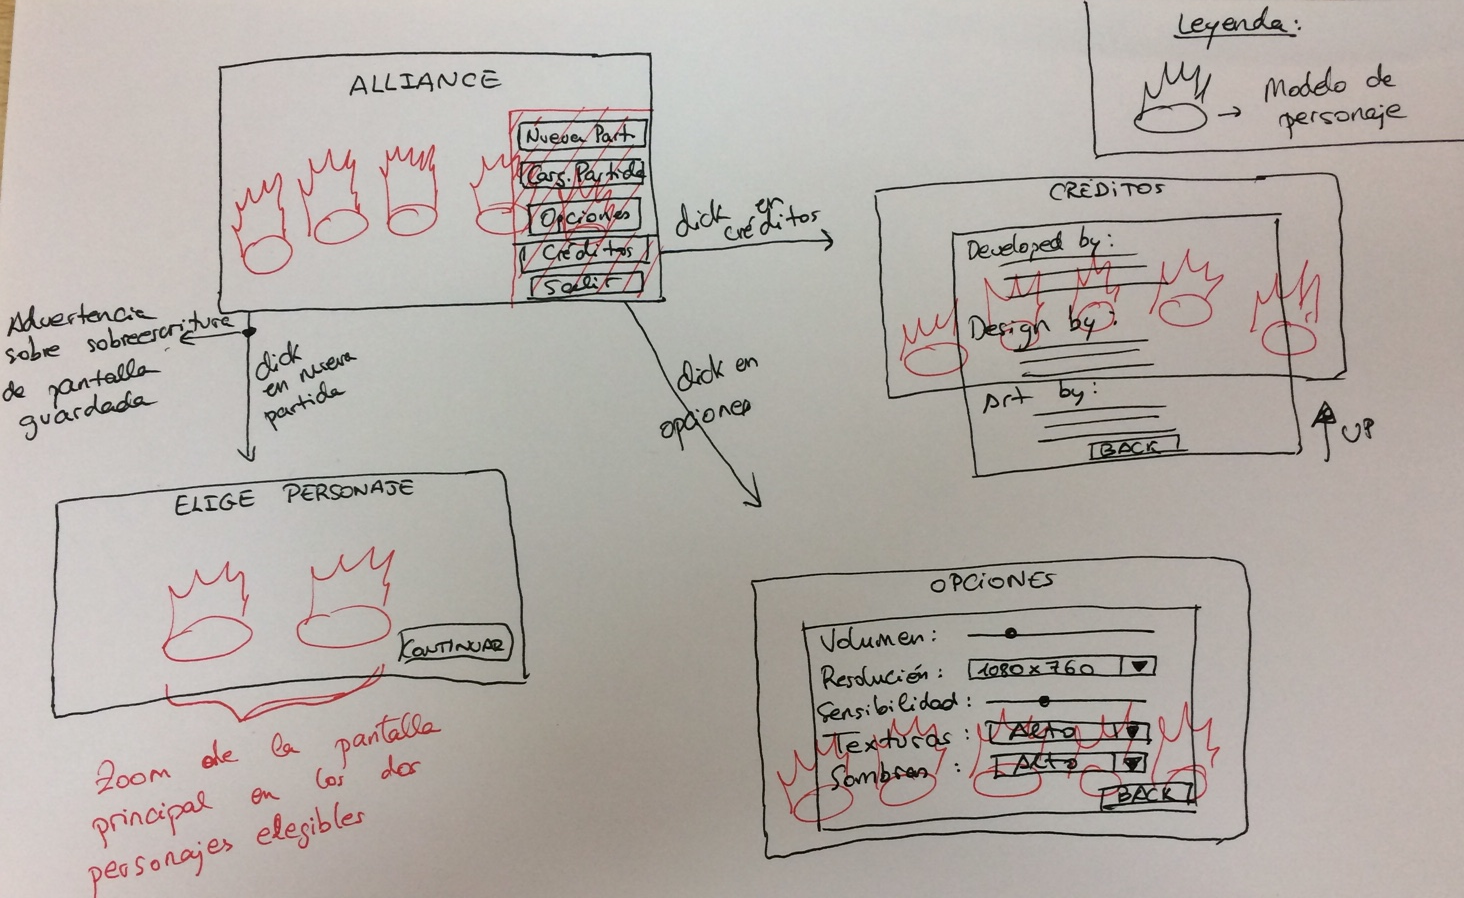
\includegraphics[width=16cm]{./images/pantallas.png}


\end{document}
